\section{1174054 - Aulyardha Anindita}

\subsection{Teori}
\begin{enumerate}
\item Mengapa file suara harus dilakukan MFCC\\
File suara harus dilakukan MFCC karena nilai-nilai pada MFCC meniru pendengaran manusia dan mereka biasanya digunakan dalam aplikasi pengenalan suara serta genre musik yang dideteksi. Nah, nilai-nilai MFCC ini kemudian akan dimasukkan langsung kedalam jaringan saraf agar dapat diubah menjadi bentuk vektor, sehingga dapat digunakan pada machine learning, karena machine learning hanya mengerti bilangan vektor. gambarannya seperti, ketika kita akan menggunakan file suara dalam machine learning, contohnya seperti melihat jam. nah machine learning ini tidak memahami rekaman suara tersebut melainkan vektornya, maka rekaman tersebut akan diubah terlebih dahulu kedalam bentuk vektor kemudian vektor tersebut akan menyesuaikan dengan kata-kata yang telah disediakan.
\hfill\break
	\begin{figure}[H]
		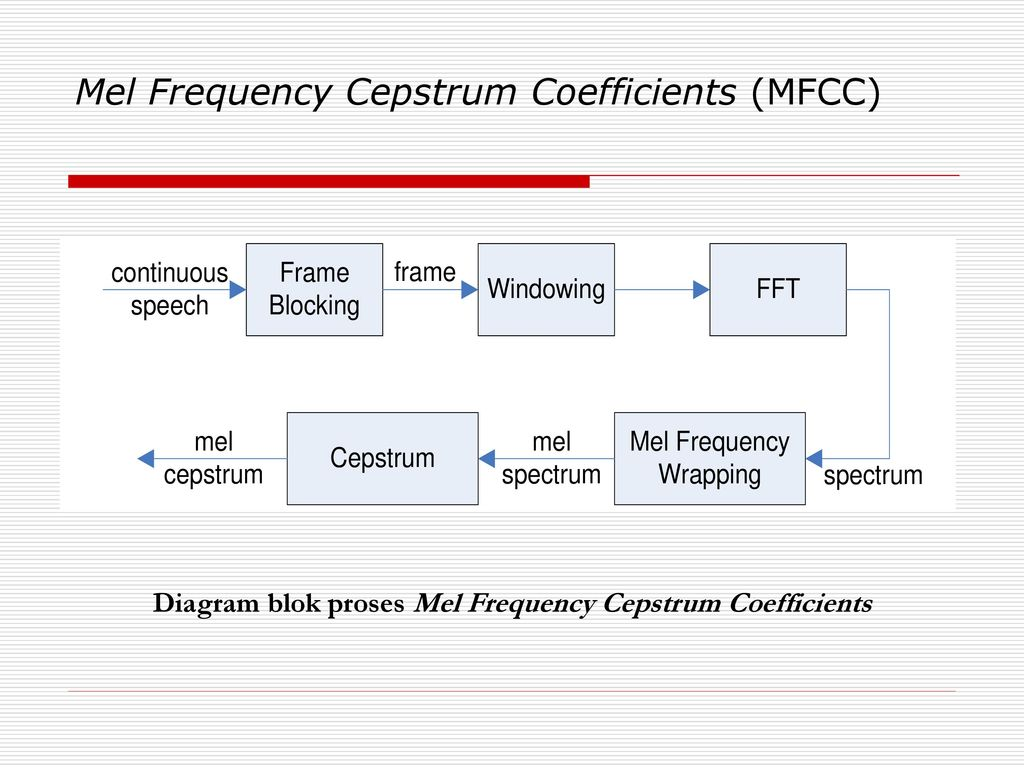
\includegraphics[width=4cm]{figures/1174054/6/1.jpg}
		\centering
		\caption{File suara MFCC}
	\end{figure}

\item Konsep Dasar Neural Network\\
Neural Network adalah suatu model yang terinspirasi tentang bagaimana neuron dalam otak manusia bekerja, nah tiap neuron pada manusia akan saling behrubungan dan informasi tersebut akan mengalir dari setiap neuron tersebut. tiap neuron tersebut akan menerima input dan melakukan operadi dot dengan sebuah weight, kemudian menjumlahkannya dan menambahkan bias, dan hasil dari operasi tersebut akan dijadikan parameter dari activation function yang akan dijadikan output dari neuron tersebut. berikut adalah contoh proses dari neural network :
\hfill\break
	\begin{figure}[H]
		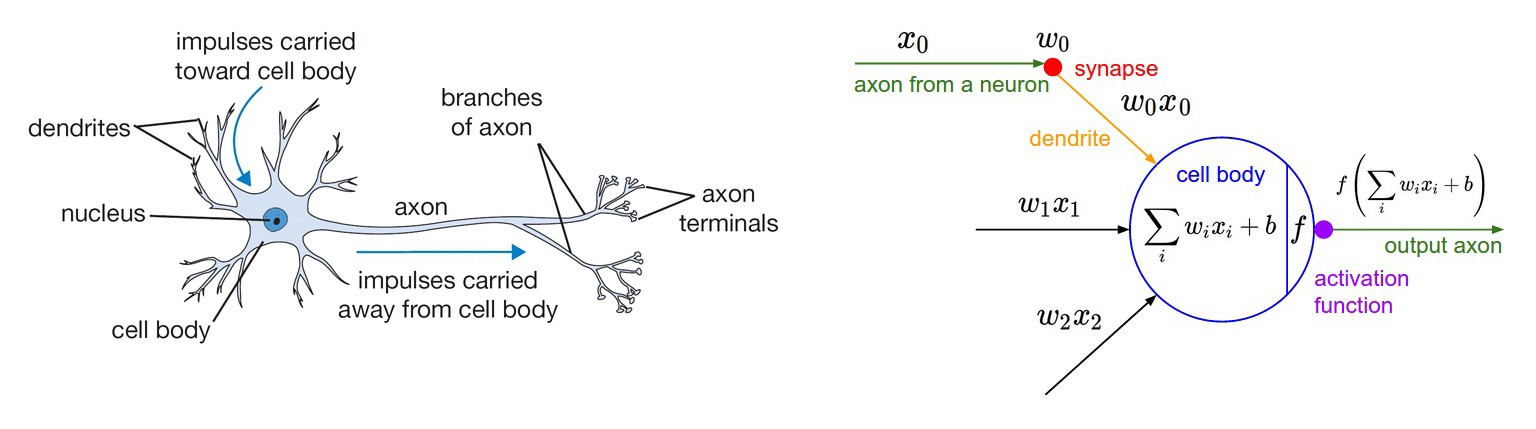
\includegraphics[width=4cm]{figures/1174054/6/2.jpeg}
		\centering
		\caption{Neural Network}
	\end{figure}

\item Konsep pembobotan dalam neural network\\
Dalam neural network terdapat jaringan yang saling berhubungan atar node-node atau simpulnya dimana pada tiap-tiap hubungan tersebut memiliki bobot koneksi yang dilatih untuk mencapai respon yang diinginkan. masing-masing bobot koneksi dipropagasikan kesuluruh simpul atau node. dengan pelatihan terhadap data berdasarkan bobot koneksi tersebut mampu memperoleh output yang diinginkan.struktur artificial neural network terdiri dari 3 lapisan. masing-masing lapisan diberikan pembobot yang akan mentransformasi nilai input menjadi nilai output. proses learning terjadi pada saat pengaturan pembobotan dan bias. Dalam metode yang dipilih, pembobotan diatur untuk meminimalisasi nilai kuadrat beda antara output model dan output taksiran atau secara umum disebut sebagai nilai kuadrat galat atau sum of square error.
\hfill\break
	\begin{figure}[H]
		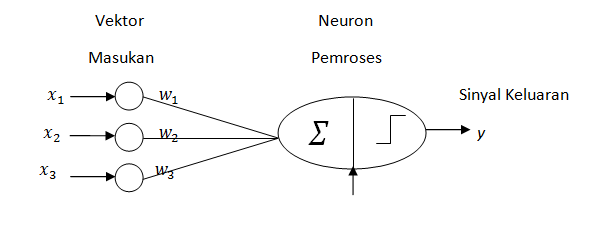
\includegraphics[width=4cm]{figures/1174054/6/3.png}
		\centering
		\caption{Pembobotan dalam Neural Network}
	\end{figure}

\item Konsep fungsi aktifasi dalam neural network\\
Fungsi activasi digunakan untuk menentukan keluaran suatu neuron. dalam fungsi aktivasi sendiri memiliki net masukan atau kombinasi linear masukan dan bobotnya. dalam fungsi aktivasi terdapat fungsi sigmoid yang kemudian dibagi dua bagian yaitu fungsi sigmoid biner dan fungsi sigmoid bipolar. adapun fungsi lain dari aktivasi yaitu memperkenalkan non-linearitas ke jaringan saraf. hal ini dapat menekan nilai dalam rentang yang lebih kecil.
\hfill\break
	\begin{figure}[H]
		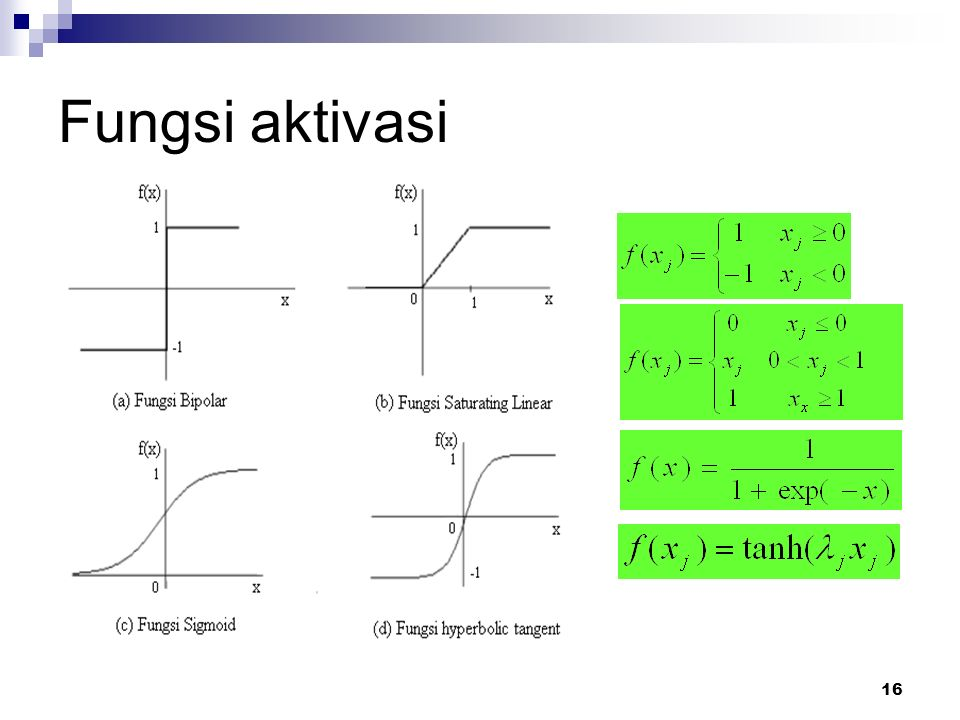
\includegraphics[width=4cm]{figures/1174054/6/4.jpg}
		\centering
		\caption{Fungsi Aktivasi}
	\end{figure}

\item Cara Membaca Hasil Plot dari MFCC\\
Dibawah ini merupakan contoh hasil plot dari rekaman suara:
\hfill\break
	\begin{figure}[H]
		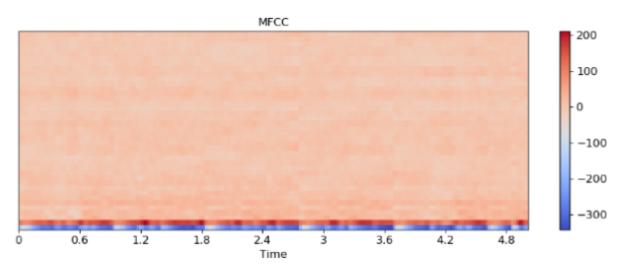
\includegraphics[width=4cm]{figures/1174054/6/5.png}
		\centering
		\caption{Membaca hasil plot dari MFCC}
	\end{figure}
dari gambar diatas dapat diketahui bahwa :
\begin{itemize}
\item terdapat 2 dimensi yaitu x sebagai waktu dan y sebagai power atau desibel
\item jika berwarna biru maka power dari suara tersebut rendah dan jika merah power dari suara tersebut tinggi
\item pada bagian atas terdapat warna merah pudar yang artinya tidak ada suara sama sekali dalam jangkauan itu.
\end{itemize}

\item One-hot encoding\\
One-hot encoding adalah suatu proses dimana variabel dikategorikal dan dikonversi menjadi bentuk yang dapat disediakan untuk algoritma ML untuk melakukan pekerjaan yang lebih baik dalam prediksi. nilai kategoris mewakili nilai numerik dari entri dalam dataset. Sebagai contoh: jika ada perusahaan lain dalam dataset, itu akan diberi nilai kategoris sebagai 4. Ketika jumlah entri unik meningkat, nilai kategoris juga meningkat secara proporsional. 0 menunjukkan tidak ada sementara 1 menunjukkan ada
\hfill\break
	\begin{figure}[H]
		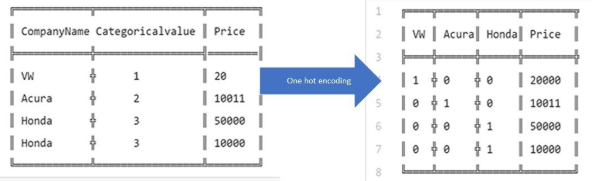
\includegraphics[width=4cm]{figures/1174054/6/6.png}
		\centering
		\caption{One-hot encoding}
	\end{figure}

\item Fungsi dari np.unique dan to.categorical dalam kode program\\
Untuk np unique berfungsi untuk menemuka elemen unik array. mengembalikan elemen unik array yang diurutkan. ada tiap output opsional selain elemen unik yaitu : indeks array input yang memberikan nilai unik, indeks array unik yang merekonstruksi array input, dan berapa kali setiap nilai unik muncul dalam array input.
\hfill\break
	\begin{figure}[H]
		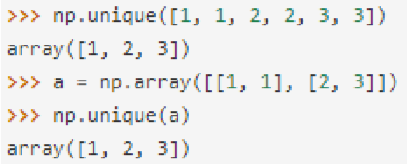
\includegraphics[width=4cm]{figures/1174054/6/7.png}
		\centering
		\caption{Numpy Unique}
	\end{figure}
sedangkan untuk to categorical berfungsi untuk mengubah vektor kelas atau integer ke matriks kelas biner.
\hfill\break
	\begin{figure}[H]
		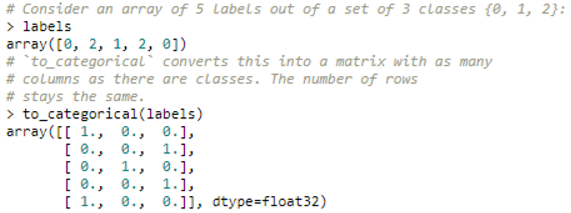
\includegraphics[width=4cm]{figures/1174054/6/8.png}
		\centering
		\caption{To Categorical}
	\end{figure}

\item Fungsi dari Sequential dalam kode program\\
Sequential berfungsi sebagai tumpukan linear lapisan. Contohnya sebagai berikut :
\hfill\break
	\begin{figure}[H]
		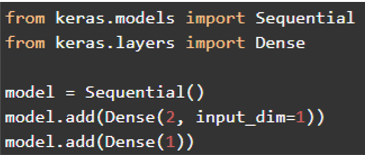
\includegraphics[width=4cm]{figures/1174054/6/9.png}
		\centering
		\caption{Sequential}
	\end{figure}

\end{enumerate}

\subsection{Praktek}
\begin{enumerate}
\item Nomor 1
\lstinputlisting[firstline=10, lastline=29]{src/1174054/6/1174054.py}
Dalam kode diatas menjelaskan isi data GTZAN. GTZAN merupakan suatu kumpulan data yang berisi 10 genre lagu dimana masing-masing genre tersebut memiliki 100 lagu yang akan dilakukan proses MFCC dan freesound yang berisi konten lagu. Dan jika GTZAN memiliki beberapa genre freesound hanya untuk satu lagu sehingga disini letak fungsinya adalah membaca file audio dan outputnya sebagai plot. Dan hasilnya bisa dilihat pada gambar berikut :
\hfill\break
	\begin{figure}[H]
		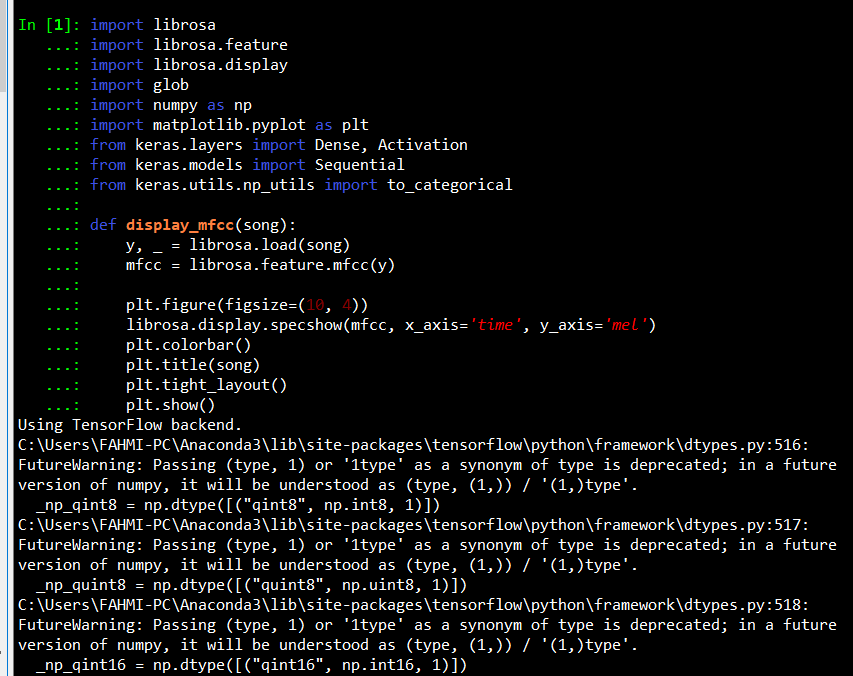
\includegraphics[width=4cm]{figures/1174054/6/10.png}
		\centering
		\caption{Hasil Nomor 1}
	\end{figure}

\item Nomor 2
\hfill\break
	\lstinputlisting[firstline=30, lastline=51]{src/1174054/6/1174054.py}
Dalam kode diatas digunakan untuk menampilkan hasil dari proses mfcc yang sudah dibuat pada nomor satu, yaitu display mfcc() yang kemudian akan menampilkan plot dari pembacaan file audio. Untuk hasil plotnya bisa dilihat pada gambar berikut:
\hfill\break
	\begin{figure}[H]
		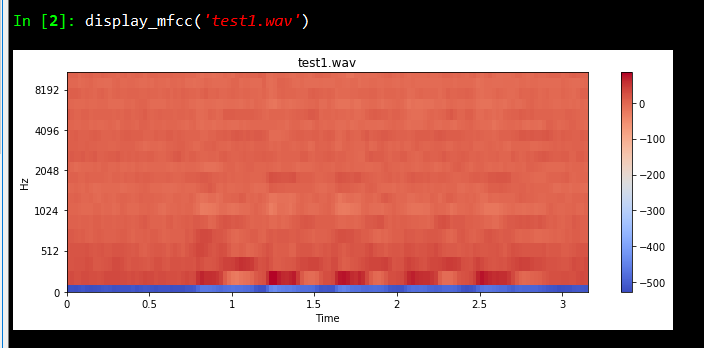
\includegraphics[width=4cm]{figures/1174054/6/11.png}
		\centering
		\caption{Hasil Nomor 2 - 1}
	\end{figure}
	\begin{figure}[H]
		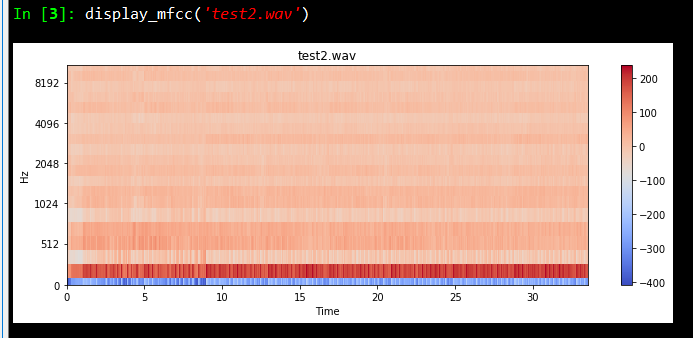
\includegraphics[width=4cm]{figures/1174054/6/12.png}
		\centering
		\caption{Hasil Nomor 2 - 2}
	\end{figure}
	\begin{figure}[H]
		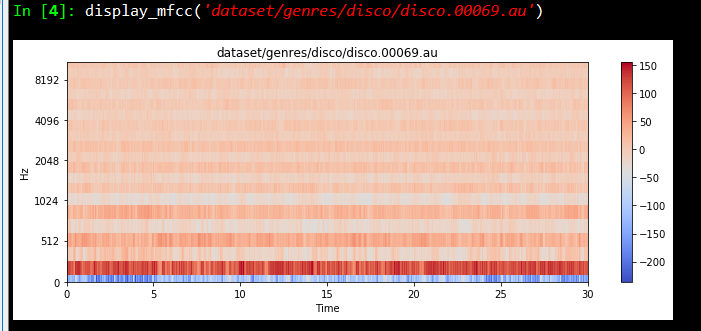
\includegraphics[width=4cm]{figures/1174054/6/13.png}
		\centering
		\caption{Hasil Nomor 2 - 3}
	\end{figure}
	\begin{figure}[H]
		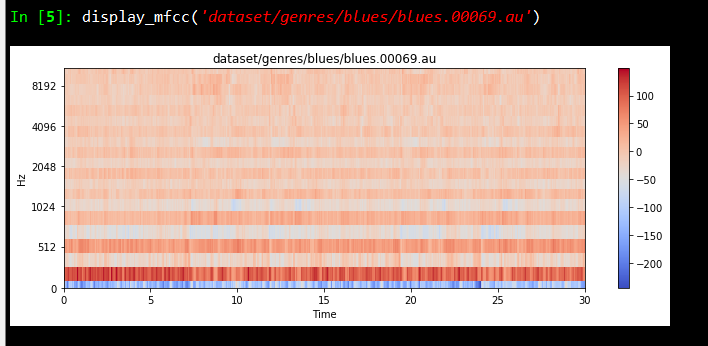
\includegraphics[width=4cm]{figures/1174054/6/14.png}
		\centering
		\caption{Hasil Nomor 2 - 4}
	\end{figure}
	\begin{figure}[H]
		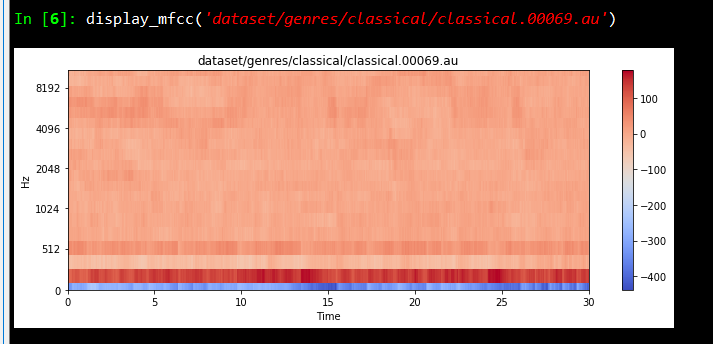
\includegraphics[width=4cm]{figures/1174054/6/15.png}
		\centering
		\caption{Hasil Nomor 2 - 5}
	\end{figure}
	\begin{figure}[H]
		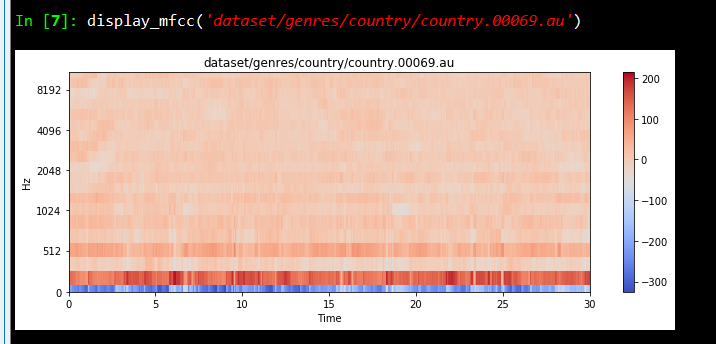
\includegraphics[width=4cm]{figures/1174054/6/16.png}
		\centering
		\caption{Hasil Nomor 2 - 6}
	\end{figure}
	\begin{figure}[H]
		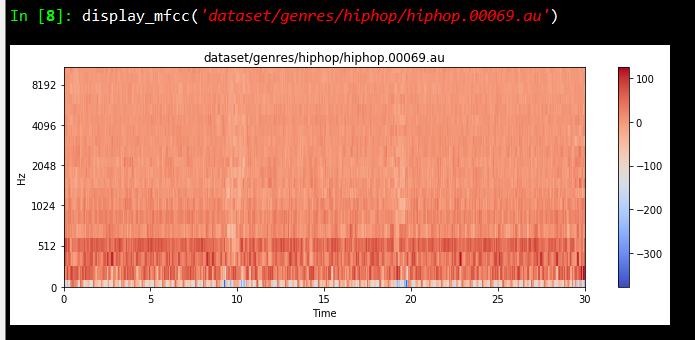
\includegraphics[width=4cm]{figures/1174054/6/17.png}
		\centering
		\caption{Hasil Nomor 2 - 7}
	\end{figure}
	\begin{figure}[H]
		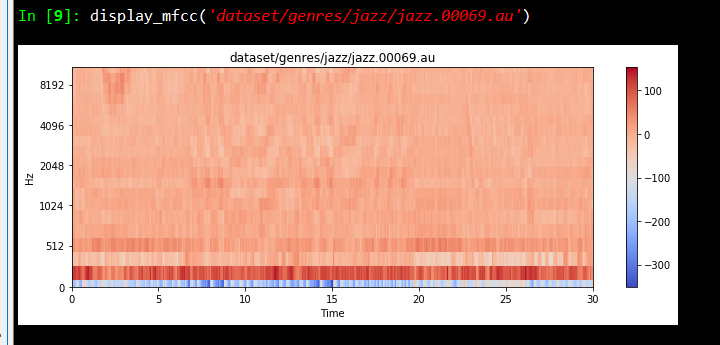
\includegraphics[width=4cm]{figures/1174054/6/18.png}
		\centering
		\caption{Hasil Nomor 2 - 8}
	\end{figure}
	\begin{figure}[H]
		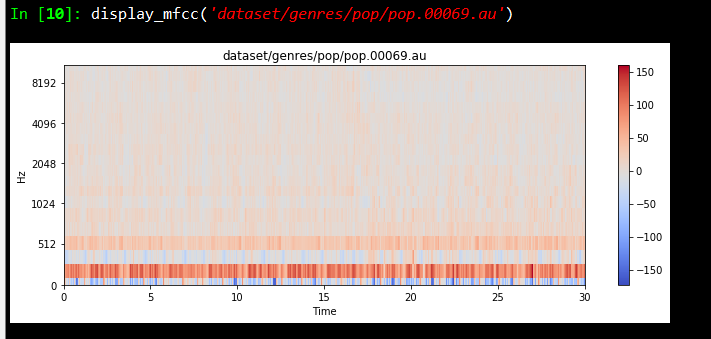
\includegraphics[width=4cm]{figures/1174054/6/19.png}
		\centering
		\caption{Hasil Nomor 2 - 9}
	\end{figure}
	\begin{figure}[H]
		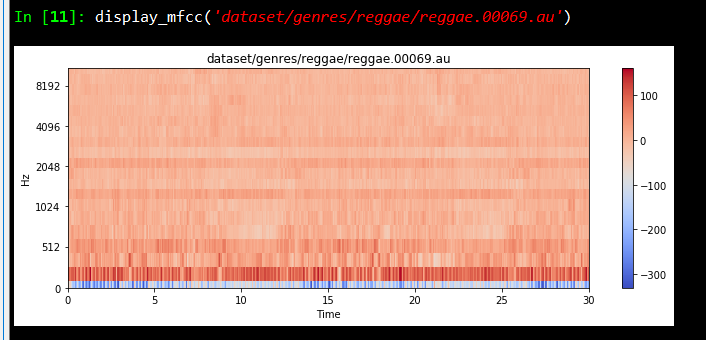
\includegraphics[width=4cm]{figures/1174054/6/20.png}
		\centering
		\caption{Hasil Nomor 2 - 10}
	\end{figure}
	\begin{figure}[H]
		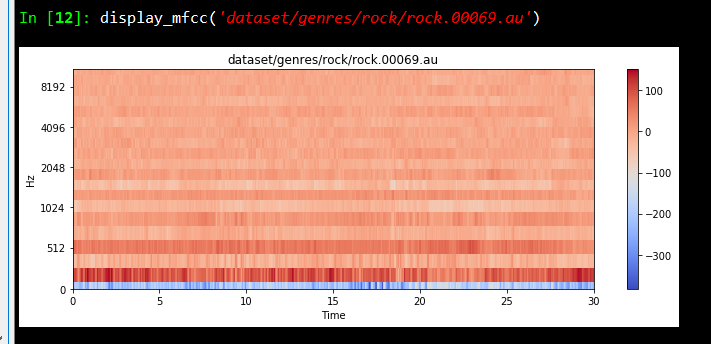
\includegraphics[width=4cm]{figures/1174054/6/21.png}
		\centering
		\caption{Hasil Nomor 2 - 11}
	\end{figure}
	
\item Nomor 3
\hfill\break
	\lstinputlisting[firstline=54, lastline=62]{src/1174054/6/1174054.py}
Pada kode diatas terdapat beberapa fungsi yang digunakan, nah pada baris pertama itu digunakan untuk membuat fungsi extract features song(f). selanjutnya, pada baris kedua digunakan untuk meload data inputan dengan menggunakan module librosa. Selanjutnya digunakan untuk membuat sebuah fitur untuk mfcc dari y atau parameter inputan. Kemudian akan mereturn dan menjadi  array lalu akan mengambil 25000 data dari hasil vektorisasi dalam satu lagu. Hasilnya dapat dilihat pada gambar berikut :
\hfill\break
	\begin{figure}[H]
		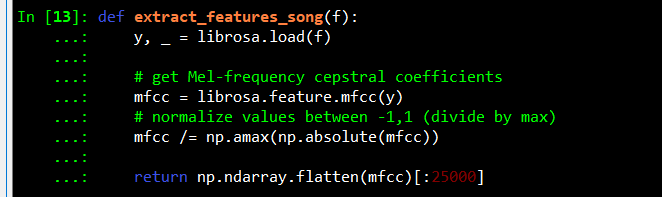
\includegraphics[width=4cm]{figures/1174054/6/22.png}
		\centering
		\caption{Hasil Nomor 3}
	\end{figure}
	
\item Nomor 4
\hfill\break
	\lstinputlisting[firstline=66, lastline=83]{src/1174054/6/1174054.py}
Dalam kode diatas digunakan kembali fungsi sebelumnya yang telah kita lakukan pada proses sebelumnya. lalu dibagian genre disesuaikan dengan dataset nama folder. Dan untuk baris selanjutnya digunakan untuk mengulang genre folder dengan ekstensi .au. lalu dipanggil fungsi ekstrak lagu. sehingga dalam setiap file dalam folder akan diekstraksi menjadi vektor dan akan ditambahkan fitur. lalu fungsi yang ditambahkan digunakan untuk menumpuk file yang telah divektorkan. Untuk hasilnya bisa dilihat pada gambar berikut :
\hfill\break
	\begin{figure}[H]
		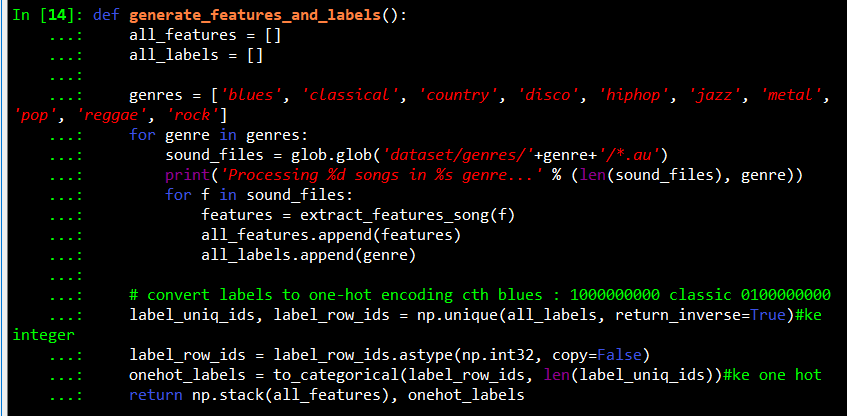
\includegraphics[width=4cm]{figures/1174054/6/23.png}
		\centering
		\caption{Hasil Nomor 4}
	\end{figure}	

\item Nomor 5
\hfill\break
	\lstinputlisting[firstline=86, lastline=91]{src/1174054/6/1174054.py}
Dalam kode diatas digunakan untuk melakukan load variabel features dan labels. Hal ini membutuhkan waktu yang lama, karena mesin akan melakukan vektorisasi terhadap semua file yang berada pada setiap folder, disini terdapat 10 folder dimana pada masing-masing folder terdiri atas 100 buah lagu, dan setiap lagu tersebut akan dilakukan vektorisasi atau ekstraksi data menggunakan mfcc. Untuk hasilnya bisa dilihat pada gambar berikut :
\hfill\break
	\begin{figure}[H]
		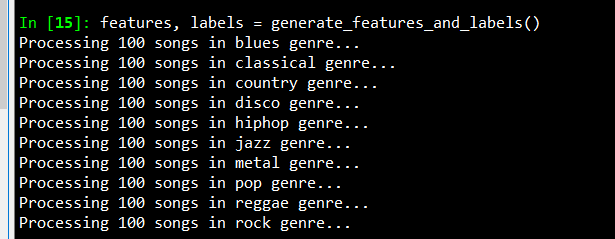
\includegraphics[width=4cm]{figures/1174054/6/24.png}
		\centering
		\caption{Hasil Nomor 5-1}
	\end{figure}
	\begin{figure}[H]
		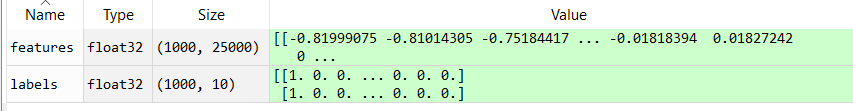
\includegraphics[width=4cm]{figures/1174054/6/25.png}
		\centering
		\caption{Hasil Nomor 5-2}
	\end{figure}
	\begin{figure}[H]
		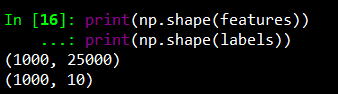
\includegraphics[width=4cm]{figures/1174054/6/26.png}
		\centering
		\caption{Hasil Nomor 5-3}
	\end{figure}
	
\item Nomor 6\\
\hfill\break
	\lstinputlisting[firstline=92, lastline=112]{src/1174054/6/1174054.py}
Dalam kode diatas digunakan untuk melakukan training split 80 persen, hal ini dilakukan agar mesin dapat terus belajar tentang data baru, jadi ketika prediksi dibuat berupa data yang terlatih mesin dapat mendapatkan persentase yang cukup bagus. Hasilnya bisa dilihat pada gambar berikut :
\hfill\break
	\begin{figure}[H]
		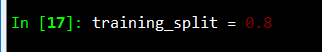
\includegraphics[width=4cm]{figures/1174054/6/27.png}
		\centering
		\caption{Hasil Nomor 6-1}
	\end{figure}
	\begin{figure}[H]
		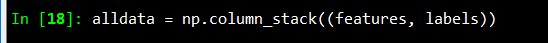
\includegraphics[width=4cm]{figures/1174054/6/28.png}
		\centering
		\caption{Hasil Nomor 6-2}
	\end{figure}
	\begin{figure}[H]
		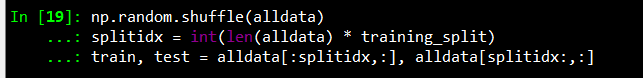
\includegraphics[width=4cm]{figures/1174054/6/29.png}
		\centering
		\caption{Hasil Nomor 6-3}
	\end{figure}
	\begin{figure}[H]
		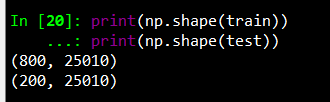
\includegraphics[width=4cm]{figures/1174054/6/30.png}
		\centering
		\caption{Hasil Nomor 6-4}
	\end{figure}
	\begin{figure}[H]
		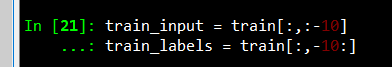
\includegraphics[width=4cm]{figures/1174054/6/31.png}
		\centering
		\caption{Hasil Nomor 6-5}
	\end{figure}
	\begin{figure}[H]
		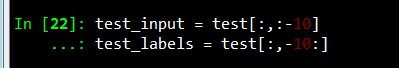
\includegraphics[width=4cm]{figures/1174054/6/32.png}
		\centering
		\caption{Hasil Nomor 6-6}
	\end{figure}
	\begin{figure}[H]
		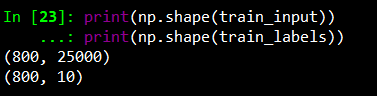
\includegraphics[width=4cm]{figures/1174054/6/33.png}
		\centering
		\caption{Hasil Nomor 6-7}
	\end{figure}
	\begin{figure}[H]
		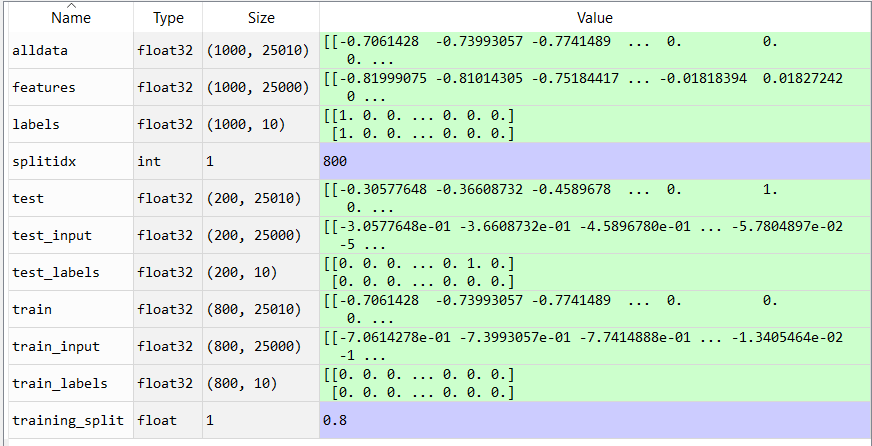
\includegraphics[width=4cm]{figures/1174054/6/34.png}
		\centering
		\caption{Hasil Nomor 6-8}
	\end{figure}
	
\item Nomor 7
\hfill\break
	\lstinputlisting[firstline=113, lastline=119]{src/1174054/6/1174054.py}
Dalam kode diatas terdapat fungsi sequential() digunakan untuk menetukan izin pada setiap neuron, yang memiliki 100 dense yang merupakan 100 neuron pertama dari data pelatihan. Fungsi dari relay itu sendiri digunakan untuk mengaktifkan neuron atau input yang memiliki nilai maksimum. sedangkan untuk dense 10 merupakan output dari hasil neuron yang berhasil diaktifkan, dan untuk dense 10 diaktifkan bisa menggunakan softmax. Hasilnya bisa dilihat pada gambar berikut :
\hfill\break
	\begin{figure}[H]
		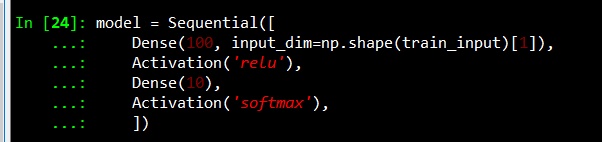
\includegraphics[width=4cm]{figures/1174054/6/35.png}
		\centering
		\caption{Hasil Nomor 7}
	\end{figure}
	
\item Nomor 8
\hfill\break
	\lstinputlisting[firstline=120, lastline=124]{src/1174054/6/1174054.py}
Dalam kode diatas terdapat model compile dimana hasilnya bisa dilihat pada gambar dibawah ini. Hasil ouput pada kode tersebut seperti gambar yang menjelaskan bahwa dense pertama memiliki 100 neurons dengan parameter sekitar 2 juta lebih dengan aktivasi 100, jadi untuk setiap neurons memiliki masing-masing 1 aktivasi. sama halnya seperti dense 2 yang memiliki jumlah neurons sebanyak 10 degan parameter 1010 dan jumlah aktifasinya 10 untuk setiap neurons tersebut dan dimana total parameternya sekitar 2,5 juta data yang akan dilatih pada mesin tersebut.
\hfill\break
	\begin{figure}[H]
		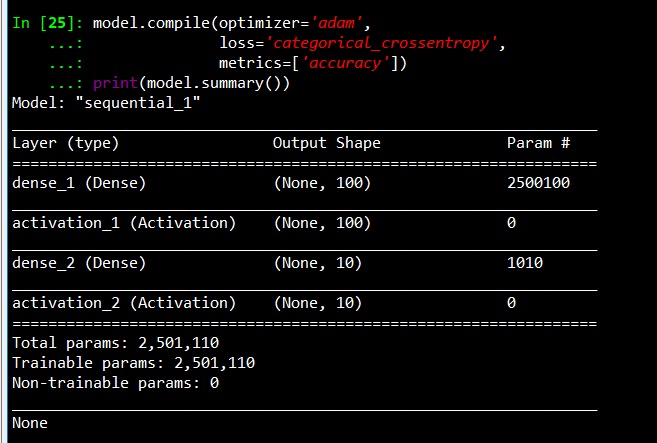
\includegraphics[width=4cm]{figures/1174054/6/36.png}
		\centering
		\caption{Hasil Nomor 8}
	\end{figure}
	
\item Nomor 9
\hfill\break
	\lstinputlisting[firstline=125, lastline=127]{src/1174054/6/1174054.py}
Dalam kode diatas digunakan untuk melatih mesin dengan data training input dan data training label. Epochs dalam kode tersebut adalah iterasi atau pengulangan berapa kali data tersebut akan dilakukan. sedangkan batch size yaitu junlah file yang akan dilakukan pelatihan pada setiap satu kali pengulangan dan terakhir validation split digunakan untuk menentukan persentase dari cross validation atau k-fold sebanyak 20 persen dari masing-masing data pengulangan. Hasilnya bisa dilihat pada gambar berikut :
\hfill\break
	\begin{figure}[H]
		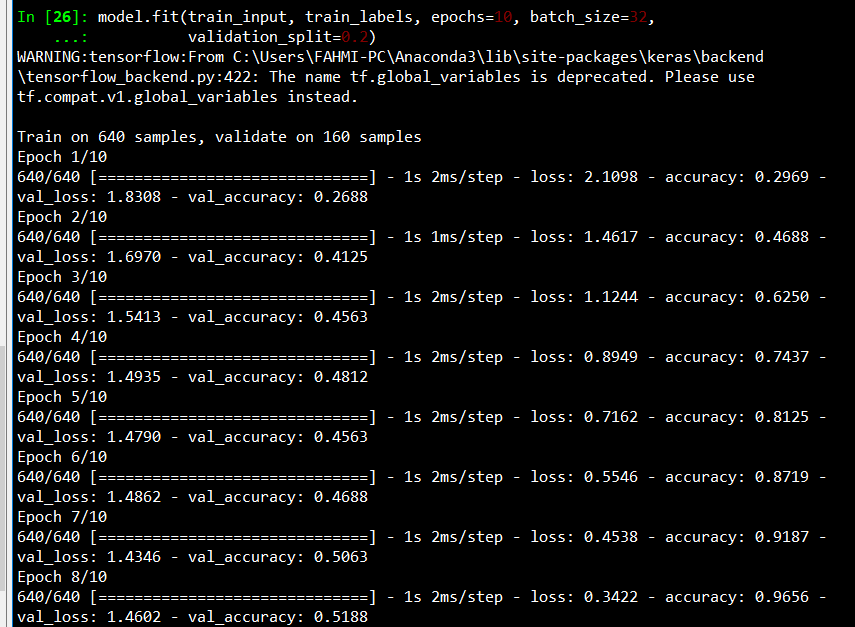
\includegraphics[width=4cm]{figures/1174054/6/37.png}
		\centering
		\caption{Hasil Nomor 9}
	\end{figure}
	
\item Nomor 10
\hfill\break
	\lstinputlisting[firstline=128, lastline=132]{src/1174054/6/1174054.py}
dalam kode diatas terdapat fungsi evaluate atau evaluasi yang digunakan untuk menguji data pengujian setiap file. disini terdapat prediksi yang hilang, artinya mesin memprediksi data, sedangkan untuk keseluruhan perjanjian sekitar 55 persen, Hasilnya bisa dilihat pada gambar berikut :
\hfill\break
	\begin{figure}[H]
		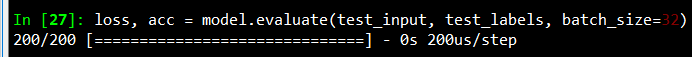
\includegraphics[width=4cm]{figures/1174054/6/38.png}
		\centering
		\caption{Hasil Nomor 10-1}
	\end{figure}
	\begin{figure}[H]
		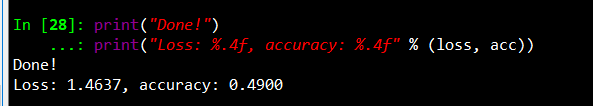
\includegraphics[width=4cm]{figures/1174054/6/39.png}
		\centering
		\caption{Hasil Nomor 10-2}
	\end{figure}
	
\item Nomor 11
\hfill\break
	\lstinputlisting[firstline=134, lastline=135]{src/1174054/6/1174054.py}
Dalam kode diatas terdapat fungsi predict, fungsi ini berfungsi untuk menghasilkan suatu nilai yang sudah iprediksi dari data training sebelumnya. dalam gambar dibawah ini, menjelaskan file yang dijalankan tersebut termasuk kedalam genre apa, hasilnya bisa dilihat pada gambar tersebut serta persentase yang paling besar yakni genre rock, maka lagu tersebut termasuk kedalam genre rock dengan perbandingan persentase hasil prediksi. Hasilnya bisa dilihat pada gambar berikut :
\hfill\break
	\begin{figure}[H]
		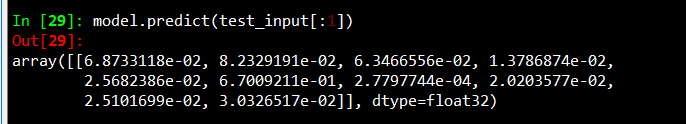
\includegraphics[width=4cm]{figures/1174054/6/40.png}
		\centering
		\caption{Hasil Nomor 11}
	\end{figure}
	
\end{enumerate}

\subsection{Penanganan Error}
\begin{enumerate}
\item ScreenShoot Error
	\begin{figure}[H]
		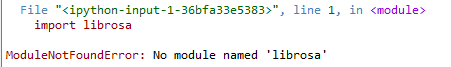
\includegraphics[width=4cm]{figures/1174054/6/error1.png}
		\centering
		\caption{Module Not Found Error}
	\end{figure}

	\item Tuliskan Kode Error dan Jenis Error
	\begin{itemize}
		\item Module Not Found Error

	\end{itemize}
	\item Cara Penanganan Error
	\begin{itemize}
		\item Module Not Found Error
		\hfill\break
		Error terjadi karena belum menginstal package atau library librosa Untuk mengatasinya dengan mengisntal library librosa pada anaconda
	\end{itemize}
\end{enumerate}


\subsection{Bukti Tidak Plagiat}
\begin{figure}[H]
	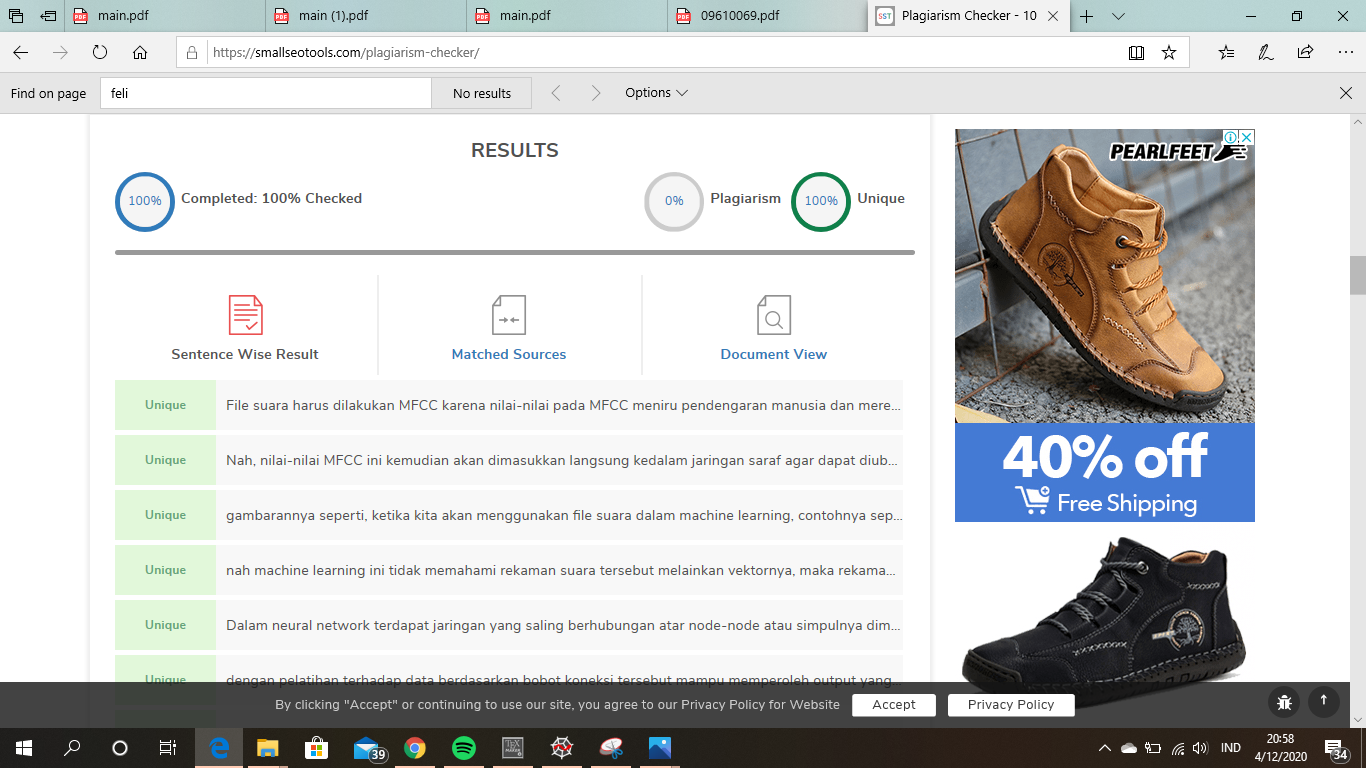
\includegraphics[width=4cm]{figures/1174054/6/plagiarisme.png}
	\centering
	\caption{Bukti Plagiasrisme}
\end{figure}

\subsection{Link Youtube}
https://youtu.be/2YVDpPMuNG0